\documentclass[11pt, a4paper]{article}

\usepackage{hyperref}
\usepackage{indentfirst}
\usepackage{graphicx}
\usepackage{float}
\graphicspath{ {img/} }
\usepackage{multicol}
\setlength{\columnsep}{0.5cm}

% \usepackage{minted} 
\usepackage{fancyhdr}
\pagestyle{fancy}
\chead{Computer Architecture 2015 Fall}
\rhead{Project 1}
\cfoot{\thepage}

\usepackage{graphicx}

\title
{
	Simple CPU with Pipeline
}
\author
{
  Chen, Chia-sheng\\
  B03902003
  \and
  Liu, Yen-ting\\
  B03902036
  \and
  Chao, Yi-ying\\
  B03902104
}
\date{\today}

\begin{document}
\maketitle

\section{Overall structure}

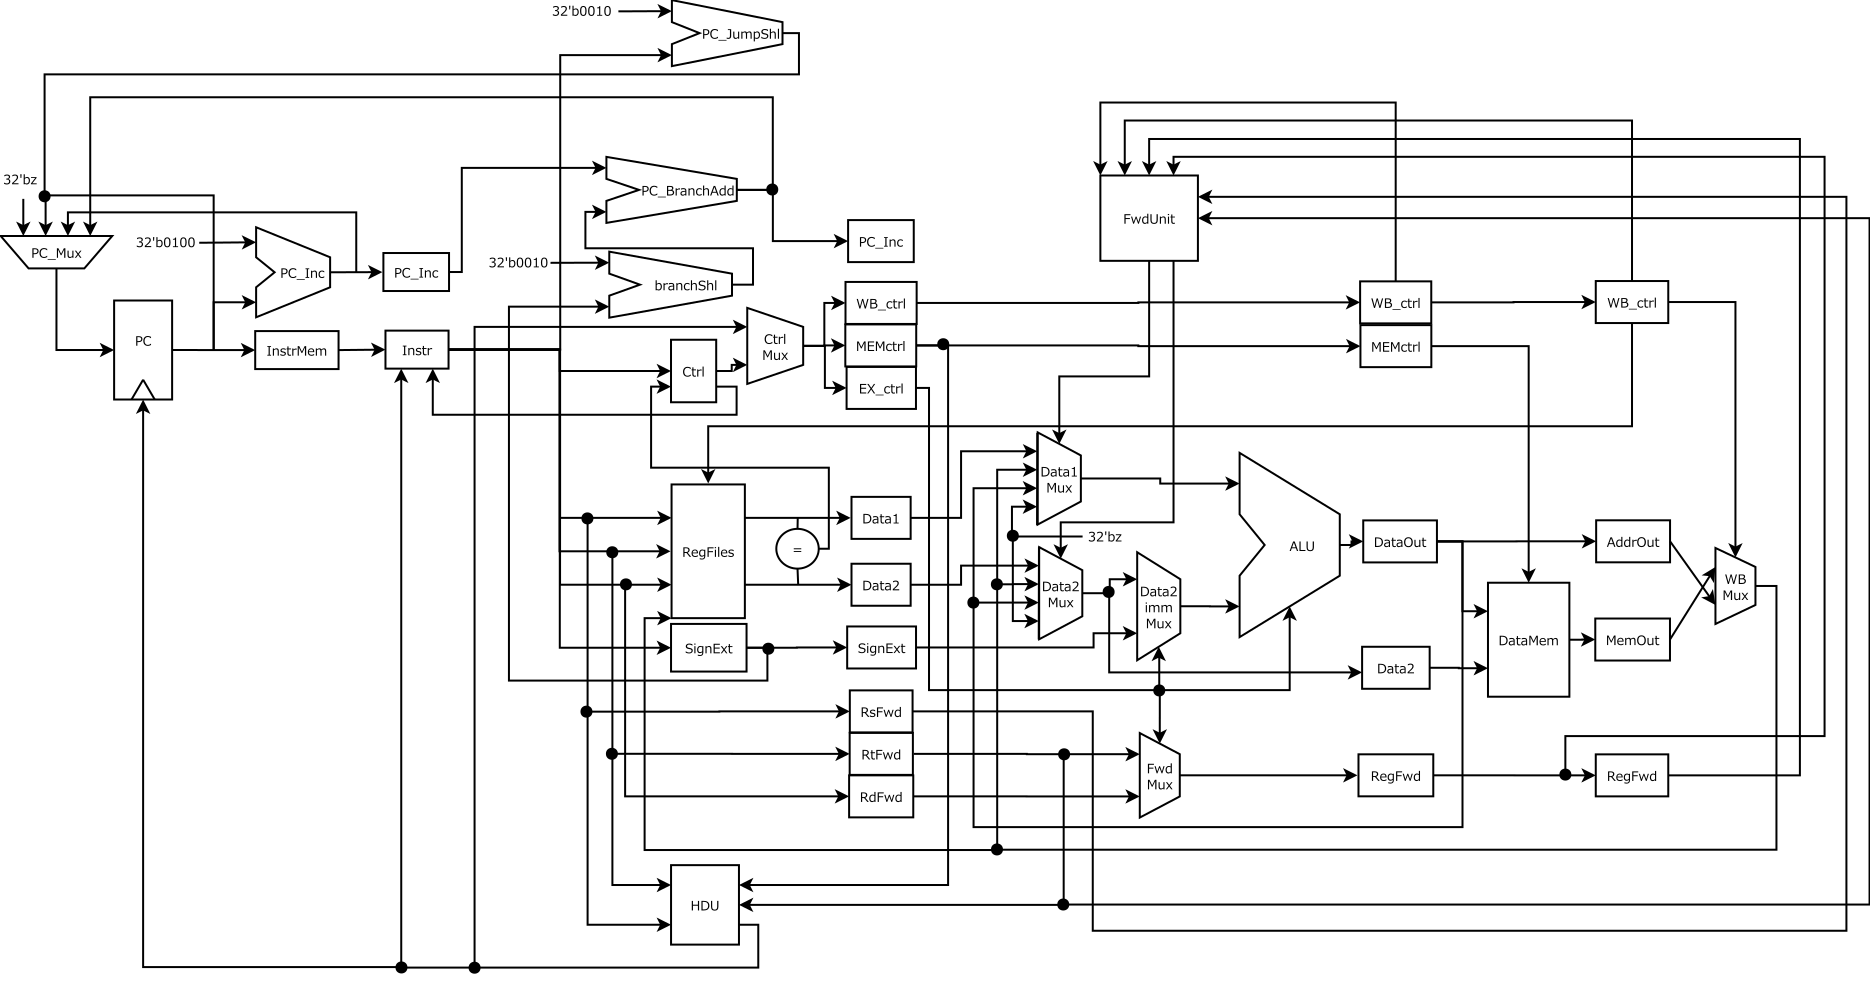
\includegraphics[width=\textwidth]{project1}
This is the overview of the structure.

\subsection{Requirements}
The entire system is based on a simplified MIPS architecture. Register file contains 32 registers, with 1KBytes of instruction memory and 32Bytes of data memory.\\

Two types of hazard handling shall be implemented: data hazard and control hazard.
\begin{itemize}
\item \textbf{Data hazard} uses {\sc forwarding unit} to reduce or avoid the stall cycles, but forwarding to {\sc ID} stage isn't necessary. 
\item \textbf{Control hazard} should contain pipeline flush, and let the instructions follow by beq or j instruction to stall for 1 cycle if necessary.
\end{itemize}

% todo Not finish yet.

\subsection{Coding guideline}

\subsection{Instruction fetch}
\par For program counter multiplexer, there are four ways to go. The first is to add 4 to current address, which is to fetch the next line. The second is to add immediate of branch instructions if specific condition was met. The third is the jump instrction. And the last one is stall.

\subsection{Instruction decode}
\par We use the standard MIPS decode method and a look up table to record and map the corresponding code to behavior.

\subsubsection{Instruction set}
\par There are 10 instructions we have to implement, they are grouped into their respective types below. 

\begin{table}[h]
	\centering
	\begin{tabular}{|c|ccc|}
	\hline
    Instruction & Type & Op & Func\\
    \hline
    and & R & 000000 & 100100 \\
    or & R & 000000 & 100101 \\
    add & R & 000000 & 100000 \\
    sub & R & 000000 & 100010 \\
    mul & R & 000000 & 011000 \\
    lw & I & 100011 & - \\
    sw & I & 101011 & - \\
    beq & I & 000100 & - \\
    j & J & 000010 & - \\
    addi & I & 001000 & - \\
    \hline
	\end{tabular}
\end{table}

Note: Since the TAs require us to test the result using the program provided, which also limits the way how OpCodes are assigned.\\


\subsection{Execution}
\par The main purpose of this section is to prepare all the data needed for ALU, and execute them. The data are either from register or forwarding from EX/MEM gate or MEM/WB gate. Forwarding unit are the signals controller of picking the data. Noticed that data could be stalled if special signal are received. 

\subsection{Memory}
\par There are two signals from MEM\_Ctrl of EX/MEM gate. One is $memread$, another $memwrite$, responsible for read and write respectively. For lw/sw instructions, DataOut is the address and Data2 the value.

\subsection{Write back}
It is possible for the CPU to write back to Data\_Mux, which is the input of ALU, or the register files. While accessibility of Data\_Mux are controlled by forwarding unit, the accessibility of register files are controlled by general control.

\subsection{Pipeline}
\par Pipeline design is the major topic of this project.As the requirement indicates, we divide the CPU datapath into five major stages, which are IF/ID/EX/MEM/WB. Following the requirement, we build corresponding registers.

\section{Modules}
\subsection{Constants}
Normally, we would hard coded the lookup table in each module, but we decide to implement it in a separated module file, and {\sc include} that module file whenever needed. This way, we can control all the reference values in a single location without constantly jumping between different files.


\subsection{Multiplexers}
We implement general two-way multiplexer and general four-way multiplexer.By assigning the width of datapath as parameter, we can reuse the same module in our design.

\subsection{Registers}
We design a latch as a general register and it's equipped with reset signal($rst$),control signal($en$),edge triggering($clk$).The latch is similar to a D flip-flop.

\subsubsection{Register files}
We assign 32 (32bits-wide) registers as the top level storage of CPU.

\subsubsection{Program counter}
\par We implement $jump$ and $branch$ with an additional 4-way multiplexer.
\par The first input (data1) is the default add setting (pc=pc+4). The second input (data2) is the Hi-Z. The third input is taken when there's a jump instruction. And the last input is preserve for branch taken.
\par In addition, there's a control signal for stall($WriteEnable$). Which allows program counter to pause for a while.

\subsection{Memories}
\par We have a general memory box for the sake of implementing following memory boxes. The general memory box gets $addr$ and provides value of the specifit $addr$.
\par The interface also contains a signal $cs$ for read enable, and another $we$ for write enable.
\par Both memory boxes gain signals from general control.
\subsubsection{Instructor memory}
We simply build a 32-by-1024-size memory for this. 

\subsubsection{Data memory}
The memory sized 32-by-32. The input $addr$ comes from $EXMEM\_ALU\_out$.

\subsection{ALU}
The main calculation module, in this project, there's a major ALU (which can be modified from the previous hw4) and some adder for branch.

\subsubsection{Comparator}
We construct a general comparator, which supports three types of comparation.\\
Given input a and b, there're three output:\\
(1)$(a>b)?$\\
(2)$(a<b)?$\\
(3)$(a==b)?$\\
To implement $beq$ instruction, we need the judgement of $a==b$, and link the result of equality to general control. The general control unit would sign the correct mux control to pc. 

\subsubsection{Sign extended}
Simply we reuse the sign extended module from the previous hw4.


\subsection{Control units}
\subsubsection{General control}
In general control, we construct a look-up table which records every instruction and its control signal accordingly.

\subsubsection{ALU control}
Since the instructions are limited , we combine the ALU control into general control, which generates the ALU control signal to ALU.

\subsubsection{Hazard detection unit}
As for hazard detection unit, we refer to textbook p.302, the logical condition is 
if
$
 (ID/EX.MemRead \,\,\&\&\,\, ((ID/EX.Rt == IF/ID.Rs)\,
 or \,(ID/EX.Rt == IF/ID.Rt))) 
$
, then stall the pipeline. How to stall the pipeline? We output stall signal which allow us to set the $IF/ID register$ and $PC$ to the origin value.

\subsubsection{Forwarding control unit}
\par Since we need to deal with data hazard, we implement forwarding control unit. Forwarding unit would check EX-hazard and MEM-hazard, which is the following cases:
\par (1) EX-hazard
\begin{itemize}
\item $if (EXMEM\_wb \,\,\&\&\,\, (EXMEM\_Rd != 0)\,\,\&\&\,\,(EXMEM\_Rd == IDEX\_Rs))$
\item $if (EXMEM\_wb \,\,\&\&\,\, (EXMEM\_Rd != 0) \,\,\&\&\,\, (EXMEM\_Rd == IDEX\_Rt))$
\end{itemize}
\par (2) MEM-hazard
\begin{itemize}
\item $if (MEMWB\_wb \,\&\&\, (MEMWB\_Rd != 0) \,\&\&\, !((EXMEM\_wb \,\&\&\, (EXMEM\_Rd != 0)) \,\&\&\, (EXMEM\_Rd == IDEX\_Rs)) \,\&\&\, (MEMWB\_Rd == IDEX\_Rs))$
\item $if (MEMWB\_wb \,\&\&\, (MEMWB\_Rd != 0) \,\&\&\, !((EXMEM\_wb \,\&\&\, (EXMEM\_Rd != 0)) \,\&\&\, (EXMEM\_Rd == IDEX\_Rt)) \,\&\&\, (MEMWB\_Rd == IDEX\_Rt))$
\end{itemize}
\par If the previous case fits, the forwarding control unit would drive the multiplexer to direct the proper value to the input of ALU.


\section{Evaluation}
\subsection{Timing sequence verification}
\begin{figure}[H]
\includegraphics[width=\textwidth]{addi}
\caption{Verify the ALU function properly, tested using {\sc addi}, {\sc add}}.
\end{figure}
\begin{figure}[H]
\includegraphics[width=\textwidth]{pipeline}
\caption{Verify the pipeline stages and the forwarding unit can function properly.}
\end{figure}
\begin{figure}[H]
\includegraphics[width=\textwidth]{flush}
\caption{Verify that the flush control pulled from the general control can function properly.}
\end{figure}
\begin{figure}[H]
\includegraphics[width=\textwidth]{stall}
\caption{Verify that the stall signal from the HDU can functino properly.}
\end{figure}

\subsection{Test bench}
The test benches are only written for critical components, which are {\sc 4-way multiplexers}, {\sc latch}, and {\sc memory}. Please reference the source code on GitHub for more details.

\subsection{Fibonacci}
This is the last measure the we've tried to verify that our code can function properly -- by running the fibonacci program provided by the TA. The \textit{correct} answer is calculated by hand, and compare it with the generated result through memory dump in the ModelSim.

\section{Work}
\subsection{Difficulties}

\paragraph{Latch cycle delay}
Due to the design of latch and the positive-edge triggering, we found that there's a inevitable cycle delay (unless we change the design of latch). The delay is from the difference of input/output of Latch, i.e., IF/ID Latch.

\paragraph{Positive-edge and negative-edge triggering}
Since we try to achieve less delay and the following bugs, we try to change positive-edge triggering into negative-edge triggering. It's reasonable to use negative-edge triggering, since it guarantees every combinational logic can be done before the reg takes data at falling edge. This avoid unpredicable hazard and make the situation predicable.

\paragraph{Debug using single steps}
Single-step through is the most common way for programmer to debug programs. However, in this case, debugging modules that can execute parallely using single-step isn't efficient. We move toward printf-style debug method with tons of waveform output to get the job done.

\subsection{Workload}
The github repo is \url{https://github.com/liuyenting/CA-Project}
\paragraph{Chia-sheng Chen}
	\begin{itemize}
		\item Draw schematics by haaaaaaaaaands ($\leftarrow$ time comsuming).
		\item Human emulator.
		\item Tracing bug.
		\item Report writing.
	\end{itemize}
\paragraph{Yen-ting Liu}
	\begin{itemize}
	\item CPU structure design.
	\item Basically, all the code you've seen on the GitHub.
	\item Debug. 
	\end{itemize}
\paragraph{Yi-ying Chao}
	\begin{itemize}
	\item Forwarding unit and Hazard detection.
	\item Report writing.
	\end{itemize}

\section{Referenc}
\begin{itemize}
	\item CS352H: Computer Systems Archictecture, Topic 9: MIPS Pipeline - Hazards. Don Fussell.
	\item CS2506 Computer Organization II, Homework 8: MIPS Pipeline Forwarding Unit.
	\item CS281 Computer Organization, MIPS Arithematic and Logic Unit (ALU). DENISON.
	\item CMSC311 Instruction Format, 2013. 
	\item Pipelined Processor Design. Luke Harvey and Stephanie Spielbauer.
	\item EE471 Final Project, Designing a Single Cycle and Pipelined CPU. Cameron Forbis, Kendrick Tang, Alex Ching.
\end{itemize}

\end{document}

